\documentclass[a4paper, 12pt]{article}

\usepackage[utf8]{inputenc}
\usepackage[T1]{fontenc}
\usepackage[indonesian]{babel}
\usepackage{amsmath, amssymb, amsfonts}
\usepackage{graphicx}
\usepackage{geometry}
\usepackage{booktabs} % For better table rules
\usepackage{caption}
\usepackage{url}
\usepackage{hyperref}
\usepackage{fancyhdr} % For headers and footers
\usepackage{enumitem} % For custom lists

\geometry{
    a4paper,
    total={170mm,257mm},
    left=20mm,
    top=20mm,
    right=20mm,
    bottom=20mm,
    headheight=15pt % Added to avoid fancyhdr warning
}

\pagestyle{fancy}
\fancyhf{} % Clear all header and footer fields
\fancyhead[L]{Jurnal Sainsmat, Maret 2020, Halaman 91-102}
\fancyhead[R]{Vol. IX, No. 1}
\fancyfoot[C]{\thepage}
\renewcommand{\headrulewidth}{0.4pt}
\renewcommand{\footrulewidth}{0pt}

% Custom command for running head on subsequent pages
\newcommand{\runninghead}[1]{%
  \fancyhead[L]{#1}
  \fancyhead[R]{\thepage}
}


\title{Model SEIR Kecanduan Game Online pada Siswa di SMP Negeri 3 Makassar \\
       \vspace{0.5em}
       \large SEIR Model of Online Game Addiction on Students in Junior High School 3 Makassar}
\author{
    Syafruddin Side$^{1),*}$, Nurul Azizah Muzakir$^{1)}$, Dian Pebriani$^{1)}$, Syana Nurul Utari$^{2)}$ \\
    \small $^{1)}$Jurusan Matematika/ Program Studi Matematika, Universitas Negeri Makassar \\
    \small $^{2)}$Jurusan Psikologi / Program Studi Psikologi, Universitas Negeri Makassar \\
    \small Received 11$^{th}$ March 2020 / Accepted 24$^{th}$ March 2020 \\
    \small $^{*}$Korespondensi: \texttt{syafruddin@unm.ac.id}
}
\date{} % No date, as it's in the author block

\begin{document}

\fancypagestyle{firstpage}{
  \fancyhf{}
  \fancyhead[L]{Jurnal Sainsmat, Maret 2020, Halaman 91-102 \\ ISSN 2579-5686 (Online) ISSN 2086-6755 (Cetak) \\ \url{http://ojs.unm.ac.id/index.php/sainsmat}}
  \fancyhead[R]{Vol. IX, No. 1}
  \fancyfoot[R]{91} % Page number for the first page
  \renewcommand{\headrulewidth}{0.4pt}
}
\maketitle
\thispagestyle{firstpage}

\begin{abstract}
\noindent\textbf{ABSTRAK} \\
Penelitian ini membahas model matematika SEIR kecanduan game online. Data yang digunakan adalah data primer berupa jumlah siswa SMP Negeri 3 Makassar yang kecanduan game online yang diperoleh dengan cara membagikan angket kepada siswa. Penelitian ini dimulai dari membangun model SEIR kecanduan game online, menentukan titik keseimbangan, menganalisis kestabilan titik keseimbangan, menentukan nilai bilangan reproduksi dasar ($R_0$), melakukan simulasi model menggunakan software Maple, dan menginterpretasikan hasil simulasi. Dalam artikel ini diperoleh model matematika SEIR kecanduan game online; dua titik keseimbangan, yaitu titik keseimbangan bebas kecanduan dan titik keseimbangan kecanduan; kestabilan titik keseimbangan bebas kecanduan dan kecanduan; serta bilangan reproduksi dasar $R_0 = 0,089$ yang menunjukkan bahwa tidak terjadi penularan kecanduan dari satu individu ke individu lain.
\vspace{0.5em}

\noindent\textbf{Kata kunci:} Model Matematika, Kecanduan Game Online, Model SEIR.
\vspace{1em}

\noindent\textbf{ABSTRACT} \\
This research discuss a SEIR mathematical model of online game addiction. The data used is primary data of the number of students in Junior High School 3 Makassar who are addicted to online game which obtained by share the questionnaires to students. This research starts from constructing a SEIR model of online game addiction, determining the equilibrium point, analysing the stability of equilibrium point, determining the basic reproduction number ($R_0$), doing a simulation of model using Maple, and interpreting the result of the simulation. In this paper we obtained a SEIR mathematical model of online game addiction; two equilibrium points which are addiction free and addiction equilibrium point; the stability of addiction free and addiction equilibrium; and the basic reproduction value $R_0 = 0,089$ indicates that there is no transmission of addiction from one individual to another.
\vspace{0.5em}

\noindent\textbf{Keywords:} Mathematical Model, Game Online Addiction, SEIR Model
\end{abstract}

\clearpage
\runninghead{Model SEIR Kecanduan Game Online pada Siswa di SMP Negeri 3 Makassar}
\setcounter{page}{92}

\section{PENDAHULUAN}
Perkembangan teknologi berupa internet memberikan manfaat yang sangat besar bagi kemajuan di segala bidang kehidupan. Hari kehari internet menyuguhkan banyak penawaran yang menarik, alih-alih menggunakan internet untuk menyelesaikan tugas atau pekerjaan, kenyataannya banyak yang beralih pada \textit{game online} (Prastyo, dkk, 2017).

\textit{Game online} adalah permaian yang dimainkan secara online via internet (Syahran, 2015). \textit{Game} dengan fasilitas online via internet menawarkan fasilitas lebih dibandingkan dengan \textit{game} biasa (seperti video \textit{game}) kerena pemain bisa berkomunikasi dengan pemain lain diseluruh penjuru dunia melalui \textit{chating} (Syahran, 2015).

Di Indonesia, fenomena bermain \textit{game} sudah banyak melibatkan remaja. \textit{Game online} mendapatkan sambutan yang luar biasa, terutama bagi remaja yang duduk di bangku SMP maupun SMA. Menurut lembaga riset pemasaran asal Amsterdam, Newzoo, pada tahun 2017 terdapat 43,7 juta \textit{gamer} (56\% diantaranya merupakan laki-laki) di Indonesia. Jumlah pemain \textit{game} di Indonesia terbanyak di Asia Tenggara, yang bermain \textit{game} di telepon genggam, \textit{personal computer}, dan \textit{laptop} (Jaya, 2012).

Bermain \textit{game online} memang kegiatan yang mengasikkan, dapat mengisi waktu luang dan menghilangkan stres, namun jika intensitas bermain \textit{game} tidak dibatasi maka dapat membuat individu kecanduan. Santoso dan Purnomo (2017) mengatakan bahwa kecanduan adalah suatu aktivitas atau substansi yang dilakukan berulang-ulang dan dapat menimbulkan dampak negatif. \textit{Kecanduangame online} ditandai oleh sejauh mana seseorang \textit{bermaingamesecaraberlebihan} yang dapat berpengaruh negatif bagi pemain \textit{game} tersebut (Prastyo, dkk, 2017).

Terdapat beberapa kasus penyimpangan yang dilakukan oleh pelajar disebabkan oleh kecanduan \textit{game online} diantaranya berbohong kepada orang tua, bolos sekolah hanya untuk main \textit{game} di warnet hingga mencuri uang agar bisa bermain \textit{game online}. Lebih lanjut, Organisasi Kesehatan Dunia atau \textit{World Health Organizations} (WHO) menetapkan kecanduan \textit{game} ke dalam versi terbaru \textit{International Statistical Classification of Diseases} (ICD) sebagai penyakit gangguan mental untuk pertama kalinya. Dalam versi terbaru ICD-11, WHO menyebut bahwa kecanduan \textit{game} merupakan \textit{disorders due to addictive behavior} atau gangguan yang disebabkan oleh kebiasaan atau kecanduan (Putri, 2018).

Dengan adanya masalah mengenai kecanduan \textit{game online}, maka perlu ditemukan penyelesaian dari masalah tersebut. Salah satu cara yaitu dengan membuatkan model matematika. Model matematika merupakan sekumpulan persamaan atau pertidaksamaan yang mengungkapkan perilaku suatu permasalahan yang nyata. Model matematika dibuat berdasarkan asumsi-asumsi. Model matematika yang telah dibentuk akan dilakukan analisis, agar model yang dibuat representatif terhadap permasalahan yang dibahas (Maesaroh, 2013; Side, dkk, 2016).

Model SEIR merupakan salah satu model matematika epidemiologi yang membagi populasi menjadi empat subpopulasi, yaitu sub populasi individu berpotensi

\clearpage
\runninghead{Side (2020)}
\setcounter{page}{93}

(\textit{Susceptible}), sub populasi individu terdeteksi penyakit tetapi belum terinfeksi (\textit{Exposed}), subpopulasi individu terinfeksi (\textit{Infected}), dan subpopulasi individu sembuh dari penyakit (\textit{Recovered}) (Ansar, 2018).

Beberapa peneliti telah mengkaji model SEIR pada penularan penyakit maupun permasalahan mengenai kecanduan \textit{game online} (Side, dkk, 2017; Ermilatni, 2016; Side, 2015; Syahran, 2015). Belum ada peneliti yang membuat model matematika SEIR pada kasus permasalahan sosial seperti kecanduan \textit{game online}. Maka dari itu, penulis tertarik untuk mengkaji masalah kecanduan \textit{game online} menggunakan model matematika SEIR, dimana terdapat empat subpopulasi yaitu subpopulasi \textit{Susceptible} atau berpotensi kecanduan \textit{game online}, subpopulasi \textit{Exposed} atau mencoba bermain \textit{game online}, subpopulasi \textit{Infected} atau kecanduan \textit{game online}, dan subpopulasi \textit{Recovered} atau tidak lagi bermain \textit{game online}.

Tujuan dari penelitian ini adalah untuk membuat model matematika SEIR untuk kasus kecanduan \textit{game online} pada siswa di SMP Negeri 3 Makassar, mengetahui titik keseimbangan model dan analisis kestabilan titik keseimbangan model, melakukan simulasi model dan menginterpretasikannya, serta mengetahui solusi dari masalah kecanduan \textit{game online} pada siswa di SMP Negeri 3 Makassar.

\subsection{Titik Keseimbangan Sistem}
Titik keseimbangan adalah sebuah keadaan dari suatu sistem yang tidak berubah terhadap waktu. Jika sistem dinamika diuraikan dalam persamaan diferensial, maka titik keseimbangan dapat diperoleh dengan mengambil turunan pertama yang sama dengan nol.

Definisi 1.1 (Toaha, dkk, 2014) Titik $\mathbf{x} \in \mathbb{R}^n$ disebut titik keseimbangan (\textit{equilibrium point}) dari $\dot{\mathbf{x}} = \mathbf{f}(\mathbf{x})$ jika memenuhi $\mathbf{f}(\mathbf{x}) = \mathbf{0}$, dimana
\[
\mathbf{f}(\mathbf{x}) = \begin{bmatrix}
f_1(x_1, x_2, \dots, x_n) \\
f_2(x_1, x_2, \dots, x_n) \\
\vdots \\
f_n(x_1, x_2, \dots, x_n)
\end{bmatrix}
\]

\subsection{Analisis Kestabilan Titik Keseimbangan}
Tinjau sistem PD non-linear orde n sebagai berikut
\begin{equation} \label{eq:pd_nonlinear}
\dot{x}_i = Ax + f_i(x_1, x_2, \dots, x_n)
\end{equation}
dimana $i= 1,2, \dots, n$.

Langkah awal penyelesaian persamaan (\ref{eq:pd_nonlinear}) yakni dengan mencari titik keseimbangan. Misalkan diperoleh titik keseimbangan $(x_1^*, x_2^*, \dots, x_n^*)$, maka langkah selanjutnya mencari matriks Jacobiannya. Misalkan $G_i(x_1, x_2, \dots, x_n) = Ax + f_i(x_1, x_2, \dots, x_n)$, matriks Jacobiannya adalah
\[
A = \begin{bmatrix}
\frac{\partial G_1}{\partial x_1} & \dots & \frac{\partial G_1}{\partial x_n} \\
\vdots & \ddots & \vdots \\
\frac{\partial G_n}{\partial x_1} & \dots & \frac{\partial G_n}{\partial x_n}
\end{bmatrix}
\]

\clearpage
\runninghead{Model SEIR Kecanduan Game Online pada Siswa di SMP Negeri 3 Makassar}
\setcounter{page}{94}

Selanjutnya substitusi titik keseimbangan pada matriks Jacobi, maka diperoleh sistem yang linear sebagai berikut,
\[ \dot{u}_i = A(x_1^*, x_2^*, \dots, x_n^*)u_i \]
Penentuan kestabilan titik keseimbangan diperoleh dengan melihat nilai eigennya, yaitu $\lambda_i$ dengan $i= 1,2, \dots, n$ yang diperoleh dari $\det(A - \lambda I) = 0$.
Secara umum kestabilan titik keseimbangan mempunyai dua perilaku, yaitu:
\begin{enumerate}
    \item Stabil jika
    \begin{enumerate}[label=\alph*.]
        \item $\text{Re}(\lambda_i) < 0$ untuk setiap $i$, atau
        \item Terdapat $\text{Re}(\lambda_j) = 0$ untuk sebarang $j$ dan $\text{Re}(\lambda_i) < 0$ untuk setiap $i \neq j$.
    \end{enumerate}
    \item Tidak stabil jika terdapat paling sedikit satu $i$ sehingga $\text{Re}(\lambda_i) > 0$ (Toaha, 2014).
\end{enumerate}

\subsection{Bilangan Reproduksi Dasar}
Bilangan reproduksi dasar merupakan bilangan yang menunjukkan jumlah individu berpotensi yang dapat kecanduan \textit{game online} yang disebabkan oleh satu individu kecanduan \textit{game online}. Secara umum bilangan reproduksi dasar $R_0$ mempunyai tiga kemungkinan, yaitu:
\begin{enumerate}
    \item Jika $R_0 < 1$, maka kecanduan akan menghilang.
    \item Jika $R_0 = 1$, maka kecanduan akan menetap.
    \item Jika $R_0 > 1$, maka kecanduan akan menular.
\end{enumerate}

\section{METODE}
Penelitian yang dilakukan merupakan jenis penelitian kajian teori dan terapan, yaitu dengan mengkaji literatur-literatur mengenai pemodelan matematika serta kecanduan \textit{game online}. Data yang digunakan dalam penelitian ini adalah data primer jumlah siswa SMP Negeri 3 Makassar yang berpotensikecanduan, mulaibermain, kecanduan, dan berhentibermaingame online. Populasi dalam penelitian ini adalah seluruh siswa SMP Negeri 3 Makassar tahun ajaran 2018/2019 yang berjumlah 1194 siswa. Melihat banyaknya populasi penelitian, maka perlu ditarik sampel penelitian. Penarikan sampel dilakukan dengan teknik acak atau \textit{random sampling}, yaitu mengacak kelas populasi. Pengacakan dilakukan karena semua kelas populasi homogen, sehingga jumlah sampel yang digunakan dalam penelitian ini berjumlah 176 siswa yang terdiri dari siswa kelas 7 dan kelas 8.

Langkah-langkah yang dilakukan dalam penelitian ini adalah sebagai berikut:
\begin{enumerate}
    \item Membangun model SEIR kecanduan \textit{game online}.
    \begin{enumerate}[label=\alph*.]
        \item Menentukan asumsi, variabel, dan parameter yang digunakan untuk model SEIR.
        \item Membentuk model SEIR kecanduan \textit{game online}.
    \end{enumerate}
    \item Menganalisis model SEIR kecanduan \textit{game online}.
    \begin{enumerate}[label=\alph*.]
        \item Menentukan titik keseimbangan model SEIR.
        \item Menentukan jenis kestabilan titik keseimbangan berdasarkan nilai eigen.
        \item Menentukan bilangan reproduksi dasar ($R_0$).
    \end{enumerate}
\end{enumerate}

\clearpage
\runninghead{Side (2020)}
\setcounter{page}{95}

\begin{enumerate}[resume]
    \item Melakukan simulasi model SEIR kecanduan \textit{game online} menggunakan software Maple.
    \begin{enumerate}[label=\alph*.]
        \item Mengumpulkan data siswa SMP Negeri 3 Makassar yang kecanduan \textit{game online} dengan cara membagikan angket kepada siswa.
        \item Menginput data siswa kecanduan \textit{game online}.
        \item Menginput hasil analisis model ke dalam software.
        \item Menganalisis hasil simulasi.
        \item Menarik kesimpulan.
    \end{enumerate}
\end{enumerate}

\section{HASIL DAN PEMBAHASAN}
\subsection{Model SEIR Kecanduan \textit{Game Online}}
Dalam penelitian ini, populasi dalam model dibagi menjadi empat kelas, yaitu kelas \textit{Susceptible} (S) yaitu berpotensi kecanduan \textit{game online}, kelas \textit{Exposed} (E) yaitu mencoba bermain \textit{game online}, kelas \textit{Infected} (I) yaitu kecanduan \textit{game online}, dan kelas \textit{Recovered} (R) yaitu berhenti bermain \textit{game online}.

Terdapat beberapa asumsi yang digunakan dalam membuat model, yaitu:
\begin{enumerate}
    \item Terdapat siswa yang memiliki \textit{game online} di gadgetnya dan tidak memiliki \textit{game online} di gadgetnya.
    \item Laju siswa yang tidak memiliki \textit{game online} di gadgetnya dianggap konstan.
    \item Siswa yang masuk kelas berpotensi kecanduan (\textit{Susceptible}) adalah mereka memiliki \textit{game online} di gadgetnya.
    \item Siswa yang masuk kelas mencoba bermain \textit{game online} (\textit{Exposed}) adalah mereka yang mulai bermain \textit{game online} dengan intensitas waktu yang normal (maksimal 2-3 jam sehari) atas dasar kemauan sendiri.
    \item Siswa yang masuk kelas kecanduan (\textit{Infected}) adalah mereka yang secara terus menerus bermain \textit{game online}; tidak akan berhenti bermain hingga merasa puas; tidak bisa lepas dari bermain \textit{game online}; tidak menghiraukan masalah kesehatan seperti waktu tidur, kebersihan badan maupun pola makan; tidak menghiraukan hubungan interpersonalnya.
    \item Siswa yang masuk kelas berhenti bermain \textit{game online} (\textit{Recovered}) adalah mereka yang sadar akan dampak negatif bermain \textit{game online} secara berlebihan dan mencari aktivitas lain yang lebih positif dan bermanfaat.
    \item Siswa yang kecanduan jika diberikan penanganan berupa pengawasan orang tua serta bimbingan dan konseling akan sembuh.
\end{enumerate}

\clearpage
\runninghead{Model SEIR Kecanduan Game Online pada Siswa di SMP Negeri 3 Makassar}
\setcounter{page}{96}

Skema model SEIR kecanduan \textit{game online} dapat dilihat pada Gambar \ref{fig:skema}.

\begin{figure}[h!]
    \centering
    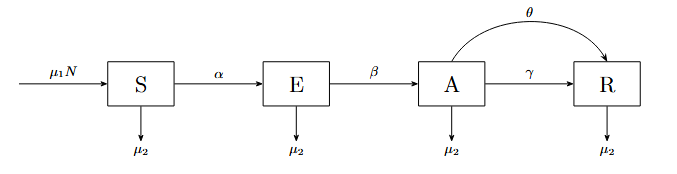
\includegraphics[width=0.8\linewidth]{diagram.png} % Replace with actual image
    \caption{Skema model SEIR kecanduan \textit{game online}}
    \label{fig:skema}
\end{figure}

Gambar \ref{fig:skema} juga dapat ditafsirkan ke dalam model matematika yang merupakan persamaan diferensial nonlinear seperti berikut:
\begin{subequations} \label{eq:seir_model}
\begin{align}
    \frac{dS}{dt} &= \mu_1 N - (\alpha + \mu_2)S \\
    \frac{dE}{dt} &= \alpha S - (\beta + \mu_2)E \\
    \frac{dI}{dt} &= \beta E - (\gamma + \theta + \mu_2)I \\
    \frac{dR}{dt} &= (\gamma + \theta)I - \mu_2 R
\end{align}
\end{subequations}
dimana N = S+E+I+R adalah total siswa yang diteliti.

\begin{table}[h!]
    \centering
    \caption{Variabel dan parameter dalam model SEIR kecanduan \textit{game online}}
    \label{tab:variabel_parameter}
    \begin{tabular}{@{}ll@{}}
        \toprule
        Variabel / Parameter & Keterangan \\
        \midrule
        S & Jumlah siswa yang berpotensi kecanduan bermain \textit{game online} \\
        E & Jumlah siswa yang mencoba bermain \textit{game online} \\
        I & Jumlah siswa yang kecanduan bermain \textit{game online} \\
        R & Jumlah siswa yang tidak lagi bermain \textit{game online} \\
        $\mu_1$ & Laju siswa yang memiliki \textit{game online} di gadgetnya \\
        $\mu_2$ & Laju siswa yang tidak memiliki \textit{game online} di gadgetnya \\
        $\alpha$ & Laju perpindahan siswa dari kelas berpotensi kecanduan \\
                 & (\textit{susceptible}) ke kelas mencoba bermain (\textit{exposed}) \\
        $\beta$ & Laju perpindahan siswa dari kelas mencoba bermain \\
                & (\textit{exposed}) ke kelas kecanduan (\textit{infected}) \\
        $\gamma$ & Laju perpindahan siswa dari kelas kecanduan (\textit{infected}) ke \\
                 & kelas tidak lagi bermain (\textit{recovered}) \\
        $\theta$ & Efektivitas pengawasan orang tua serta program \\
                 & bimbingan dan konseling pada siswa \\
        \bottomrule
    \end{tabular}
\end{table}

\clearpage
\runninghead{Side (2020)}
\setcounter{page}{97}

\subsection{Analisis Model SEIR Kecanduan \textit{Game Online}}
\subsubsection{Penentuan titik keseimbangan}
Akan dicari titik keseimbangan berdasarkan sistem persamaan (\ref{eq:seir_model}). Titik keseimbangan terjadi pada saat $(\frac{dS}{dt}, \frac{dE}{dt}, \frac{dI}{dt}, \frac{dR}{dt}) = (0,0,0,0)$. Sistem persamaan (\ref{eq:seir_model}) memiliki dua titik keseimbangan, yaitu titik keseimbangan bebas kecanduan $E_0$ dan titik keseimbangan kecanduan $E_\epsilon$. Titik keseimbangan bebas kecanduan diperoleh dengan asumsi bahwa $E = 0$ dan $I = 0$ yang berarti tidak ada individu yang kecanduan dan tidak ada penanganan. Berdasarkan sistem persamaan (\ref{eq:seir_model}), diperoleh titik keseimbangan bebas kecanduan $E_0(S, E, I, R) = (\frac{\mu_1 N}{\mu_2+\alpha}, 0,0,0)$. Untuk titik keseimbangan kecanduan, diperoleh $E_\epsilon(S, E, I, R) = (S^*, E^*, I^*, R^*)$ dimana
\begin{align*}
    S^* &= \frac{\mu_1 N}{\mu_2+\alpha} \\
    E^* &= \frac{\alpha \mu_1 N}{(\mu_2+\beta)(\mu_2+\alpha)} \\
    I^* &= \frac{\beta \alpha \mu_1 N}{(\mu_2+\gamma+\theta)(\mu_2+\beta)(\mu_2+\alpha)} \\
    R^* &= \frac{(\gamma+\theta)\beta \alpha \mu_1 N}{\mu_2(\mu_2+\gamma+\theta)(\mu_2+\beta)(\mu_2+\alpha)}
\end{align*}

\subsubsection{Penentuan jenis kestabilan titik keseimbangan}
Jenis kestabilan titik keseimbangan bebas kecanduan $E_0$ diperoleh dengan melakukan pelinearan pada sistem persamaan (\ref{eq:seir_model}) disekitar $E_0$, sehingga diperoleh matriks Jacobian sebagai berikut.
\[
J(E_0) = \begin{pmatrix}
-\alpha - \mu_2 & 0 & 0 & 0 \\
\alpha & -\beta - \mu_2 & 0 & 0 \\
0 & \beta & -\gamma - \theta - \mu_2 & 0 \\
0 & 0 & \gamma + \theta & -\mu_2
\end{pmatrix}
\]
Untuk mengetahui kestabilan $E_0$, maka dicari nilai eigen dari matriks $J(E_0)$ dengan menentukan $\det(J(E_0) - \lambda I) = 0$, dimana $\lambda$ adalah nilai eigen dan $I$ adalah matriks identitas.
\[
\det \begin{pmatrix}
-\alpha - \mu_2 - \lambda & 0 & 0 & 0 \\
\alpha & -\beta - \mu_2 - \lambda & 0 & 0 \\
0 & \beta & -\gamma - \theta - \mu_2 - \lambda & 0 \\
0 & 0 & \gamma + \theta & -\mu_2 - \lambda
\end{pmatrix} = 0
\]
Diperoleh nilai eigen yaitu $\lambda_1, \lambda_2, \lambda_3, \lambda_4$ dengan $\lambda_1 = -\alpha - \mu_2$, $\lambda_2 = -\beta - \mu_2$, $\lambda_3 = -\gamma - \theta - \mu_2$, $\lambda_4 = -\mu_2$. Karena $\alpha, \mu_2, \beta, \gamma, \theta$ bernilai positif maka bagian real dari keempat nilai eigen tersebut adalah negatif sehingga titik keseimbangan bebas kecanduan $E_0$ bersifat stabil.

Selanjutnya menentukan jenis kestabilan titik keseimbangan kecanduan $E_\epsilon$ dengan cara yang sama seperti menentukan jenis kestabilan titik keseimbangan bebas kecanduan $E_0$. Sehingga diperoleh nilai eigen yaitu $\lambda_1 = -\alpha - \mu_2$, $\lambda_2 = -\beta - \mu_2$, $\lambda_3 = -\gamma - \theta - \mu_2$, $\lambda_4 = -\mu_2$. Karena $\alpha, \mu_2, \beta, \gamma, \theta$ bernilai positif maka bagian real dari keempat nilai eigen tersebut adalah negatif sehingga titik keseimbangan kecanduan $E_\epsilon$ bersifat stabil.

\clearpage
\runninghead{Model SEIR Kecanduan Game Online pada Siswa di SMP Negeri 3 Makassar}
\setcounter{page}{98}

\subsubsection{Bilangan reproduksi dasar}
Bilangan reproduksi dasar dapat ditentukan menggunakan metode \textit{next generation matrix} dari sistem persamaan (\ref{eq:seir_model}). Pada model matematika tersebut, kelas kecanduan \textit{game online} adalah \textit{infected} (I) sehingga persamaan diferensial yang digunakan adalah:
\[ \frac{dI}{dt} = \beta E - (\gamma + \theta + \mu_2)I \]
Misalkan $\mathcal{F} = \beta E$ dan $\mathcal{V} = (\gamma + \theta + \mu_2)I$. $\mathcal{F}$ dan $\mathcal{V}$ dilinearisasi diperoleh
\[ F = \beta, \quad V = (\gamma + \mu_2 + \theta) \quad \text{dan} \quad V^{-1} = \frac{1}{\gamma+\mu_2+\theta} \]
\textit{Next generation matrix} diperoleh dari hasil perkalian $F$ dan $V^{-1}$ sebagai berikut:
\[ K = FV^{-1} = \beta \left( \frac{1}{\gamma + \theta + \mu_2} \right) \]
Maka diperoleh $R_0 = \frac{\beta}{\gamma+\theta+\mu_2}$.

\subsection{Simulasi Model SEIR Kecanduan \textit{Game Online}}
Simulasi dilakukan menggunakan software Maple 18 dan dengan memberikan nilai untuk masing-masing parameter. Nilai-nilai parameter yang diambil sehingga diperoleh $R_0 = 0,089 < 1$ disajikan pada Tabel \ref{tab:simulasi_parameter}. $R_0 < 1$ mengindikasikan bahwa tidak terjadi penularan kecanduan dari satu individu ke individu lain. Selanjutnya diberikan nilai awal siswa yang masuk kelas berpotensi $S(0)$ adalah 72 siswa, siswa yang masuk kelas mencoba bermain $E(0)$ adalah 77 siswa, siswa yang masuk kelompok kecanduan $I(0)$ adalah 18 siswa, dan siswa yang masuk kelompok tidak lagi bermain $R(0)$ adalah 9 siswa. Total siswa yang diteliti (N) adalah 176.

\begin{table}[h!]
    \centering
    \caption{Nilai parameter dalam model SEIR kecanduan \textit{game online}}
    \label{tab:simulasi_parameter}
    \begin{tabular}{@{}lc@{}}
        \toprule
        Parameter & Nilai \\
        \midrule
        $\mu_1$ & 0,409 \\
        $\mu_2$ & 0,097 \\
        $\alpha$ & 0,438 \\
        $\beta$ & 0,102 \\
        $\gamma$ & 0,051 \\
        $\theta$ & 1 \\
        \bottomrule
    \end{tabular}
    \caption*{\footnotesize Sumber: Hasil olahan data Tahun 2019}
\end{table}

Simulasi model SEIR tanpa pengawasan orang tua serta program bimbingan dan konseling dapat dilihat pada Gambar \ref{fig:plot_tanpa_pengawasan} sebagai berikut.

\clearpage
\runninghead{Side (2020)}
\setcounter{page}{99}

\begin{figure}[h!]
    \centering
    \includegraphics[width=0.8\linewidth]{placeholder_plot1.png} % Replace with actual image
    \caption{Plot model SEIR tanpa pengawasan orang tua serta bimbingan dan konseling pada siswa}
    \label{fig:plot_tanpa_pengawasan}
    \caption*{\centering \footnotesize
    \begin{tabular}{@{}ll@{}}
    $\bullet$ Susceptible & $\bullet$ Exposed \\
    $\bullet$ Recovered & $\bullet$ Infected
    \end{tabular}}
\end{figure}

Pada Gambar \ref{fig:plot_tanpa_pengawasan} terlihat bahwa jumlah siswa yang berpotensi kecanduan pada awal pengamatan adalah 72 orang dan diperkirakan akan bertambah setiap bulannya hingga bulan ke 36 mencapai kurang lebih 135 orang. Jumlah siswa yang mencoba bermain \textit{game online} pada awal pengamatan adalah 77 orang dan diperkirakan akan bertambah setiap bulannya hingga bulan ke 36 mencapai kurang lebih 290 orang. Jumlah siswa yang kecanduan \textit{game online} pada awal pengamatan adalah 18 orang dan diperkirakan akan bertambah setiap bulannya hingga bulan ke 36 mencapai 200 orang. Jumlah siswa yang tidak lagi bermain \textit{game online} pada awal pengamatan adalah 9 orang dan diperkirakan akan bertambah setiap bulannya hingga bulan ke 36 mencapai kurang lebih 95 orang.

Simulasi model SEIR dengan pengawasan orang tua serta program bimbingan dan konseling dapat dilihat pada Gambar \ref{fig:plot_dengan_pengawasan} sebagai berikut.

\begin{figure}[h!]
    \centering
    \includegraphics[width=0.8\linewidth]{placeholder_plot2.png} % Replace with actual image
    \caption{Plot model SEIR dengan pengawasan orang tua serta bimbingan dan konseling pada siswa}
    \label{fig:plot_dengan_pengawasan}
    \caption*{\centering \footnotesize
    \begin{tabular}{@{}ll@{}}
    $\bullet$ Susceptible & $\bullet$ Exposed \\
    $\bullet$ Recovered & $\bullet$ Infected
    \end{tabular}}
\end{figure}

\clearpage
\runninghead{Model SEIR Kecanduan Game Online pada Siswa di SMP Negeri 3 Makassar}
\setcounter{page}{100}

Pada Gambar \ref{fig:plot_dengan_pengawasan} terlihat bahwa jumlah siswa yang berpotensi kecanduan pada awal pengamatan adalah 72 orang dan diperkirakan akan bertambah setiap bulannya hingga bulan ke 36 mencapai kurang lebih 135 orang. Jumlah siswa yang mencoba bermain \textit{game online} pada awal pengamatan adalah 77 orang dan diperkirakan akan bertambah setiap bulannya hingga bulan ke 36 mencapai kurang lebih 290 orang. Jumlah siswa yang kecanduan \textit{game online} pada awal pengamatan adalah 18 orang dan jumlahnya akan menurun pada bulan ke 2, tetapi jumlah siswa yang kecanduan akan bertambah pada bulan berikutnya hingga bulan ke 36 mencapai 26 orang. Jumlah siswa yang tidak lagi bermain \textit{game online} pada awal pengamatan adalah 9 orang dan diperkirakan akan bertambah setiap bulannya hingga bulan ke 36 mencapai kurang lebih 250 orang. Hal ini menunjukkan bahwa terjadi penurunan jumlah siswa yang kecanduan \textit{game online} jika diberikan penanganan berupa pengawasan orang tua serta bimbingan dan konseling oleh guru kepada siswa yang kecanduan, dan meningkatkan jumlah siswa yang tidak lagi bermain \textit{game online}.

\subsection{Solusi Masalah Kecanduan \textit{Game Online} pada Siswa di SMP Negeri 3 Makassar}
Berdasarkan hasil simulasi model SEIR kecanduan \textit{game online}, untuk mengurangi jumlah siswa SMP Negeri 3 Makassar yang kecanduan \textit{game online}, solusi yang peneliti tawarkan bagi pihak sekolah berupa rekomendasi, yaitu:
\begin{enumerate}
    \item Pihak sekolah menghimbau orang tua siswa agar senantiasa mengawasi anaknya dalam bermain \textit{game online}.
    \item Pihak sekolah memberdayakan program bimbingan dan konseling bagi para siswa baik yang merasa dirinya mulai kecanduan maupun yang telah kecanduan.
    \item Pihak sekolah mengadakan seminar kepada orang tua siswa tentang \textit{game online} dan masalah yang akan ditimbulkannya.
\end{enumerate}

\section{KESIMPULAN}
Berdasarkan pembahasan yang telah dilakukan, diperoleh kesimpulan sebagai berikut:
\begin{enumerate}
    \item Model matematika SEIR kecanduan \textit{game online} dapat dinyatakan sebagai berikut:
    \begin{align*}
        \frac{dS}{dt} &= \mu_1 N - (\alpha + \mu_2)S \\
        \frac{dE}{dt} &= \alpha S - (\beta + \mu_2)E \\
        \frac{dI}{dt} &= \beta E - (\gamma + \theta + \mu_2)I \\
        \frac{dR}{dt} &= (\gamma + \theta)I - \mu_2 R
    \end{align*}
    \item Model matematika SEIR kecanduan \textit{game online} menghasilkan dua titik keseimbangan, yaitu titik keseimbangan bebas kecanduan dan titik keseimbangan kecanduan yang keduanya bersifat stabil.
    \item Setelah melakukan simulasi model, diperoleh plot model tanpa penanganan dan dengan penanganan dan terdapat perbedaan pada jumlah siswa yang kecanduan \textit{game online} dan tidak lagi bermain \textit{game online} dari kedua simulasi model. Jika tidak ada penanganan sama sekali, diperkirakan jumlah siswa yang kecanduan tiga
\end{enumerate}

\clearpage
\runninghead{Side (2020)}
\setcounter{page}{101}

\begin{enumerate}[resume]
    \item[] tahun mendatang mencapai 200 orang dan jumlah siswa yang sadar akan dampak negatif bermain \textit{game online} secara berlebihan dan memilih untuk tidak lagi bermain mencapai 95 orang. Berbeda jika diberi penanganan berupa pengawasan serta bimbingan dan konseling ke guru, jumlah siswa yang kecanduan tiga tahun mendatang menurun hingga mencapai 26 orang dan jumlah siswa yang sadar akan dampak negatif bermain \textit{game online} secara berlebihan dan memilih untuk tidak lagi bermain meningkat menjadi 250 orang. Hal ini menunjukkan bahwa pengawasan orang tua serta bimbingan dan konseling sangat efektif untuk mengurangi jumlah siswa yang kecanduan serta meningkatkan jumlah siswa yang berhenti bermain \textit{game online}.
    \item Solusi permasalahan kecanduan \textit{game online} pada siswa di SMP Negeri 3 Makassar yang peneliti tawarkan adalah rekomendasi untuk pihak sekolah dalam upaya mengurangi jumlah siswa yang kecanduan \textit{game online} yaitu berupa pengawasan orang tua, program bimbingan dan konseling yang diberikan oleh guru kepada siswa, dan mengadakan seminar kepada siswa tentang \textit{game online} dan masalah yang akan ditimbulkannya.
\end{enumerate}

\section*{UCAPAN TERIMA KASIH}
Ucapan terima kasih diberikan kepada pihak Jurusan Matematika Univeristas Negeri Makassar dan pihak pemberi dana penelitian yaitu Kemristekdikti.

\section*{DAFTAR PUSTAKA}
\begin{enumerate}[label={}, itemsep=0.5em, leftmargin=0pt, itemindent=1.5em, labelwidth=*, align=left]
    \item Ansar A. 2018. \textit{Pemodelan Matematika SEIR dengan Vaksinasi pada Penyebaran Penyakit Malaria (Studi Kasus: Kabupaten Merauke)}. [Skripsi]. Makassar: Universitas Negeri Makassar.
    \item Ermilatni E. 2016. \textit{Model Matematika SEIR untuk Kontrol Campak dengan Pengaruh Vaksinasi di Kabupaten Bulukumba}. [Skripsi]. Makassar: Universitas Negeri Makassar.
    \item Jaya ES. 2012. WHO Tetapkan Kecanduan Game Sebagai Gangguan Mental, Bagaimana “Gamer” Indonesia Bisa Sembuh?. \url{https://theconversation.com/who-tetapkan-kecanduan-game-sebagai-gangguan-mental-bagaimana-gamer-indonesia-bisa-sembuh-99029}. Diakses tanggal 4 Desember 2018.
    \item Maesaroh U. 2013. \textit{Model Matematika untuk Kontrol Campak Menggunakan Vaksinasi}. [Skripsi]. Yogyakarta: Universitas Islam Negeri SunanKalijaga.
    \item PrastyoY, EosinaP, FatimahF. 2017. Pembagian Tingkat Kecanduan Game Online Menggunakan K-Means Clustering serta Korelasinya terhadap Prestasi Akademik. \textit{Jurnal Universitas Negeri Yogyakarta}, 2, 138-148.
\end{enumerate}

\clearpage
\runninghead{Model SEIR Kecanduan Game Online pada Siswa di SMP Negeri 3 Makassar}
\setcounter{page}{102}

\begin{enumerate}[label={}, itemsep=0.5em, leftmargin=0pt, itemindent=1.5em, labelwidth=*, align=left, resume]
    \item Putri GS. 2018. WHO Resmi Tetapkan Kecanduan Game Sebagai Gangguan Mental. \url{https://sains.kompas.com/read/2018/06/19/192900123/who-resmi-tetapkan-kecanduan-game-sebagai-gangguan-mental}. Diakses tanggal 10 Juni 2019.
    \item Santoso YRK, \& Purnomo JT. 2017. Hubungan Kecanduan Game Online terhadap Penyesuaian Sosial pada Remaja. \textit{Jurnal Humaniora Yayayasan Bina Darma}, 4, 27-44.
    \item Side, S. 2015. Model SEIR pada Penularan Hepatitis B. \textit{Jurnal Scientific Pinisi}, 1, 97-102.
    \item Side S, Sanusi W, Setiawan, NF. 2016. Analisis dan Simulasi Model SITR pada Penyebaran Penyakit Tuberkulosis di Kota Makassar. \textit{Jurnal Sainsmat}, 5, 191-204.
    \item SideS, Irwan, MulbarU, SanusiW. 2017. SEIR Model Simukation for Hepatitis B. \textit{Proceeding the 3$^{rd}$ Electric and Green Material International Conference (EGM) 2017}.
    \item Syahran, R. 2015. Ketergantungan Online Game dan Penanganannya. \textit{Jurnal Psikologi Pendidikan dan Konseling}, 1, 84-92.
    \item Toaha, Khaeruddin, Mansyur. 2014. Model SIR Untuk Penyebaran Penyakit Flu Burung. \textit{Jurnal Matematika, Statistika, \& Komputasi}, 10, 82-91.
\end{enumerate}

\end{document}